\documentclass[11pt,a4paper]{article}
% Reproducible build: no embedded dates and a fixed trailer id, so re-running pdflatex on the same
% sources yields the same bytes (the committed report.pdf is checked with diff, like the tables).
\pdfinfoomitdate=1
\pdftrailerid{}
\usepackage[margin=2.4cm]{geometry}
\usepackage{booktabs}
\usepackage{graphicx}
\usepackage{amsmath}
\usepackage[hidelinks]{hyperref}

\newcommand{\bps}{\,\text{bps}}

\title{Systematic futures: method comparison under one evaluation protocol}
\author{Research note}
\date{2026-09-11}

\begin{document}
\maketitle

\begin{abstract}
Sixteen CME futures roots, daily contract-level prices from 2010 to 2024Q1, six classic method
families and two LightGBM variants, one vectorised engine, one volatility overlay, one cost model and
one evaluation protocol: a pre-declared decision rule inside develop+validate, and a single
out-of-sample window read once. The headline result is negative in the useful direction: the ML
variants that win the pre-declared comparison in-sample fail it out of time, while turnover and the
diversification return decide the rest. Every number below is read from the committed result files in
\texttt{results/}; market data is not redistributed.
\end{abstract}

\section{Data and construction}
Raw per-contract daily prices for 16 CME roots from pysystemtrade's \texttt{multiple\_prices\_csv}
snapshot, pinned at commit \texttt{b4a25e6} and frozen upstream on 2024-03-28. Each row carries the
three active legs (front, successor, prior) with contract identifiers. The roll calendar is
\emph{observed} from the leg data rather than estimated; the continuous series is built by ratio
back-adjustment (at each roll, the new-to-old front ratio on the prior session rescales earlier
closes), with the invariant that the continuous series' daily return equals the held contract's own
return on every session including roll days --- pinned by test at floating-point tolerance. The basis
series is computed from raw closes as $\text{close(next)}/\text{close(front)}-1$. Every derived file
is SHA-256-gated by a committed manifest; ingest fails on drift.

\section{Method specifications}
\begin{table}[h]
\centering
\small
\begin{tabular}{@{}lll@{}}
\toprule
Family & Rule & Source \\
\midrule
Baseline & constant full-long, overlay-sized (null model) & M4 \\
TSMOM & equal-weight vol-scaled 5/10/20d + 1/3/12m horizon signs & M1, M2, S4 \\
XS momentum & centred cross-sectional rank of 12-month return & S3 \\
Carry & sign of the negative basis (long backwardated) & M3 \\
Seasonality & sign of same-calendar-month trailing score; and a $\pm50\%$ tilt on TSMOM & S4 \\
6a \texttt{ml\_defaults} & LightGBM defaults, purged/embargoed walk-forward, no search & M5--M7 \\
6b \texttt{ml\_tuned} & as 6a with a pruned TPE search per fold & M5--M7 \\
\bottomrule
\end{tabular}
\end{table}

\section{Evaluation protocol}
One accounting path (\texttt{engine.run}) for every family and every parameter search: signals in
$[-1,1]$ per symbol per day, a shared sizing overlay that scales \emph{each symbol} to a 10\% annualized
volatility target with $\pm1$ notional caps applied identically, a linear cost charge of $b$ basis points
per side on traded notional, and metrics reported at $b \in \{0,2,5,10\}$ with $b=2$ the headline level a
decision is read at. Turnover is book-level --- mean daily traded notional per unit of capital, the base
the charge is taken on --- so $b$ costs $\text{turnover} \times b \times 252 \times 10^{-4}$ of annual
return. Sharpe is annualized at $\sqrt{252}$ in both windows as a stated convention: the frozen panel
carries 309.6 sessions per year before 2022 and 258.4 after, so the two windows' Sharpe \emph{levels} are
not strictly comparable, while the DSR the rule reads is a probability and is unaffected. Sizing per
symbol is not sizing per book --- realized book volatility runs 0.9--3.0\% in develop+validate and
1.5--4.6\% out of time --- so the families are like-for-like in rule and cost, not in delivered risk.
A signal formed with data through day $t$ drives the position held from $t$ to $t+1$; a regression test
fails on a look-ahead implementation and passes on the correct convention. Develop 2010--2019 and
validate 2020--2021 form the decision window; the out-of-sample window 2022--2024Q1 is read exactly
once, at the end, by one script, with the walk-forward schedule extended across the whole panel so
that the fold covering 2022 trains entirely inside develop+validate. Reports carry Sharpe, Sortino,
maximum drawdown, turnover and the Deflated Sharpe Ratio (deflated by the configurations each
selection actually evaluated: 1 for every classic family, 100 for the tuned variant).

\section{Results}
\begin{table}[h]
\centering
\small
\begin{tabular}{@{}lrrrr@{}}
\toprule
& \multicolumn{2}{c}{Develop+validate} & \multicolumn{2}{c}{Out-of-sample} \\
\cmidrule(lr){2-3}\cmidrule(lr){4-5}
Family & Sharpe & DSR & Sharpe & DSR \\
\midrule
Baseline            & 0.408 & 0.9403 & $-0.694$ & 0.1470 \\
TSMOM (benchmark)   & $-0.085$ & 0.3726 & 0.551 & 0.7966 \\
XS momentum         & 0.406 & 0.9397 & 1.174 & 0.9611 \\
Carry               & $-3.614$ & 0.0000 & $-1.756$ & 0.0041 \\
Seasonality         & $-0.088$ & 0.3683 & 0.770 & 0.8793 \\
Seasonal tilt       & $-0.116$ & 0.3284 & 0.407 & 0.7304 \\
6a \texttt{ml\_defaults} & 0.799 & 0.9989 & 0.072 & 0.5433 \\
6b \texttt{ml\_tuned}    & 1.550 & 0.9999 & 0.390 & 0.0261 \\
\bottomrule
\end{tabular}
\caption{Sharpe and Deflated Sharpe Ratio at 2\bps/side. Pre-declared rule: an ML variant wins only
if its decision-window DSR beats the benchmark's. Both clear it in develop+validate; both fail it out
of time.}
\end{table}

\begin{table}[h]
\centering
\small
\begin{tabular}{@{}lrrrr@{}}
\toprule
Family & $0\bps$ & $2\bps$ & $5\bps$ & $10\bps$ \\
\midrule
Baseline            & 0.419 & 0.408 & 0.390 & 0.361 \\
TSMOM               & 0.200 & $-0.085$ & $-0.508$ & $-1.203$ \\
XS momentum         & 0.562 & 0.406 & 0.172 & $-0.216$ \\
Carry               & $-3.214$ & $-3.614$ & $-4.203$ & $-5.147$ \\
Seasonality         & $-0.027$ & $-0.088$ & $-0.177$ & $-0.326$ \\
Seasonal tilt       & 0.163 & $-0.116$ & $-0.530$ & $-1.208$ \\
6a \texttt{ml\_defaults} & 1.406 & 0.799 & $-0.122$ & $-1.660$ \\
6b \texttt{ml\_tuned}    & 2.074 & 1.550 & 0.746 & $-0.616$ \\
\bottomrule
\end{tabular}
\caption{Develop+validate Sharpe by cost level. Turnover is identical across a row; only the price
per trade changes. Trend, the tilt and both ML variants flip sign between gross and headline cost.}
\end{table}

\begin{figure}[h]
\centering
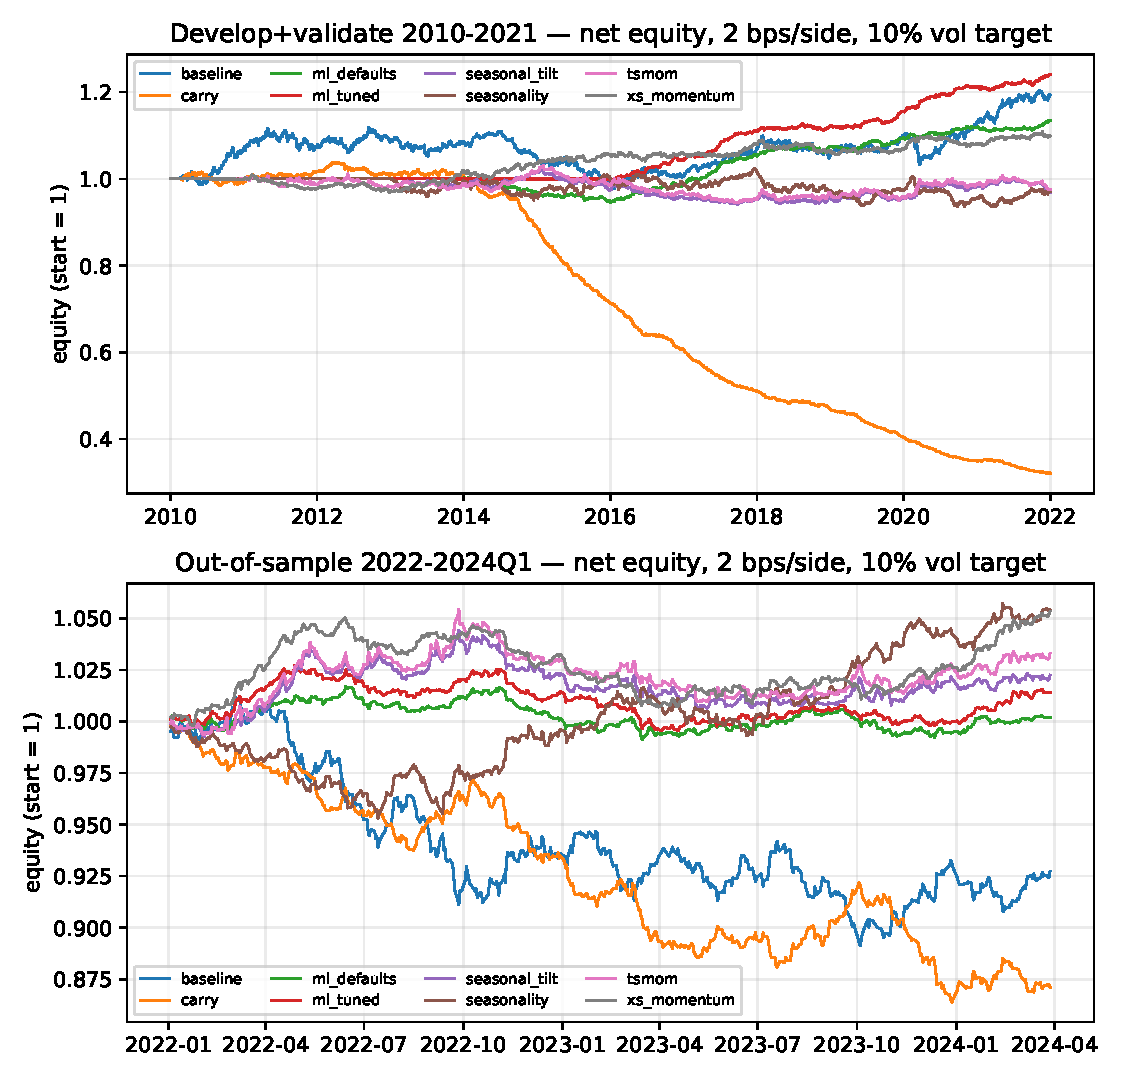
\includegraphics[width=\textwidth]{figures/equity.pdf}
\caption{Net equity at 2\bps/side, both windows, from the committed return series.}
\end{figure}

\section{Findings}
\begin{enumerate}
\item \textbf{Costs select strategies.} At $5\bps$ the survivors differ by window: develop+validate
leaves the baseline, XS momentum and the tuned variant positive, while the out-of-sample window leaves
XS momentum, seasonality, the trend benchmark and the tilt. Trend and the tilt flip sign between gross
and the headline level; both ML variants stay positive on both, at a cost of most of their signal.
\item \textbf{A null model is a real competitor.} Vol-targeted buy-and-hold earns 0.408 at $2\bps$ on
book turnover of 0.007 --- the diversification return, which any signal must beat before claiming edge.
\item \textbf{The ML result is the honest one.} In-window winners (DSR 0.9989 / 0.9999 against the
benchmark's 0.3726), out-of-time failures (0.5433 / 0.0261 against 0.7966). The in-window advantage is
concentrated in 2015--2019 and 2020--2021 --- the periods the benchmark lost money --- while 6a was
$-0.80$ in 2010--2014 and 6b had no coverage there at all. Out of time, cost consumes 6a's signal:
0.759 gross, 0.072 net, book turnover 0.199 per day.
\item \textbf{Purge and embargo guarantee no label leakage, not generalisation.} The folds are clean
by construction and asserted on every run; the features are a non-linear re-expression of the same
premia, so the protocol could not create persistence the premia do not have. A naive-split
counterfactual was deliberately not run: the size of what the protocol prevented is argued, not
measured.
\item \textbf{Standalone seasonality fails on signal, not cost} ($-0.027$ gross at book turnover 0.025,
a quarter of the benchmark's 0.103), on a score backed by five priors per calendar month.
\item \textbf{Carry's number is a frequency artefact.} The published construction is a slope magnitude
with rank weighting and monthly rebalancing; what ran here is the sign of the current basis, refreshed
daily, and that sign moves with the front leg's own price. Holding the identical signal from each
month's first session earns $+0.163$ where the daily refresh earns $-3.614$, and inverting the daily
rule earns $+2.807$ (\texttt{results/out\_of\_sample/carry\_frequency.csv}). The sign convention is \emph{not}
resolved by adopting the profitable direction, and the carry premium is neither confirmed nor refuted
by these numbers.
\item \textbf{2023 is the year nobody earned.} Out of time, every family sits at or below zero in 2023
except seasonality, while 2022 and 2024Q1 pay trend and XS momentum. The passive book loses in all
three, so what generalised was cross-sectional selection, not exposure.
\end{enumerate}

\section{Limitations}
One universe (16 CME roots), one out-of-sample window, one read. The cost model is linear and
constant --- no market impact, no bid/ask, no volume-dependent slippage. M6's CSCV
probability-of-backtest-overfitting diagnostic is not implemented; the multiple-testing discipline is
the trial-count DSR deflation plus the single out-of-sample read. Two SHOULD readings (S5, S9) and
the M7 book chapters are not read: the interpretation resting on them is marked as
scaffolded in \texttt{docs/findings/memo.md}. The ML result is specific to this feature set, label
horizon, fold geometry, cost level and window; it is not a statement about machine learning on
futures in general.

\section*{Reproducibility}
\texttt{uv sync}, fetch the pinned snapshot, rebuild derived data (manifest-gated),
\texttt{uv run python scripts/build\_families.py}, \texttt{build\_decision.py},
\texttt{build\_out\_of\_sample.py}; the committed tables are reproduced exactly. Reading order for the
story: \texttt{notebooks/analysis.ipynb}, then \texttt{docs/findings/memo.md}.

\end{document}
